\chapter{Wyznaczenie ścieżki}
\label{cha:wyznaczenieSciezki}

Wyznaczenie najkrótszych ścieżek jest jednym z podstawowych problemów w teorii grafów. Algorytmy wyszukiwania ścieżek mają wielorakie zastosowanie, począwszy od wyznaczenia najkrótszych tras na mapie, poprzez przesyłanie wiadomości przez sieć routerów, kończąc na wyznaczaniu połączeń lotniczych o najmniejszym koszcie. Wynikiem działania algorytmów wyznaczania ścieżek jest uporządkowany zbiór wierzchołków, którymi należy kolejno podążać, aby dotrzeć do wyznaczonego wcześniej celu. Podczas symulacji algorytm wykorzystywany jest w pierwszym kroku. Przed właściwym uruchomieniem symulacji zostają wyznaczone najkrótsze ścieżki prowadzące każdego z pieszych do celu, które są później podstawą do dla działania SFM.

Algorytmów wyszukiwania ścieżek jest bardzo wiele, najważniejsze z nich to:

\begin{itemize}
\item Algorytm Dijkstry - przykład algorytmu zachłannego. Jeden z najbardziej rozpowszechnionych algorytmów w dziedzinie przeszukiwania ścieżek. Jego złożoność obliczeniowa rośnie w miarę wzrostu punktów węzłowych,
\item Algorytm A* - jest to rozszerzona wersja algorytmu Dijkstry. Dzięki zastosowaniu heurystyki skraca się czas obliczeń,
\item Algorytm Bellmana-Forda - ma zastosowanie, kiedy niektóre krawędzie w grafie mają ujemne wagi
\item Algorytm Floyda-Warshalla - pozwala na odnalezienie najkrótszych ścieżek pomiędzy wszystkimi parami wierzchołków w grafie,
\item Przeszukiwanie wszerz BFS - najprostszy z algorytmów, nie uwzględnia wag ścieżek,
\item Przeszukiwanie wgłąb DFS - podobny do algorytmu BFS, wymaga mniej zasobów oraz jest szybszy.
\end{itemize}

W symulacji przeprowadzonej na potrzeby tej pracy został zastosowany Algorytm A*. Gwarantuje on zawsze znalezienie optymalnej ścieżki, jeśli tylko istnieje. Jego użycie nie wymaga także szczególnie skomplikowanych obliczeń. Algorytm A* jest znacznie szybszy w porównaniu do Algorytmu Dijkstry. Nie tylko czas wyszukiwania ścieżki jest krótszy, ale również ilość odwiedzonych elementów na mapie jest mniejsza, co skutkuję mniejszą złożonością pamięciową. W przeprowadzonych przez autora porównaniach, Algorytm A* pozwala na średnio $16 sekund$ szybsze wyszukanie ścieżki odwiedzając średnio $1710$ węzłów mniej niż Algorytm Dijkstry. Działanie algorytmów przedstawiają rysunki \ref{fig:djikstra} oraz \ref{fig:astar}. Kolor fioletowy oznacza odwiedzone węzły, zielony węzeł początkowy, a czerwony końcowy. Kolorem żółtym oznaczona została wyznaczona ścieżka.

\begin{figure}
\label{fig:djikstra}
\centering
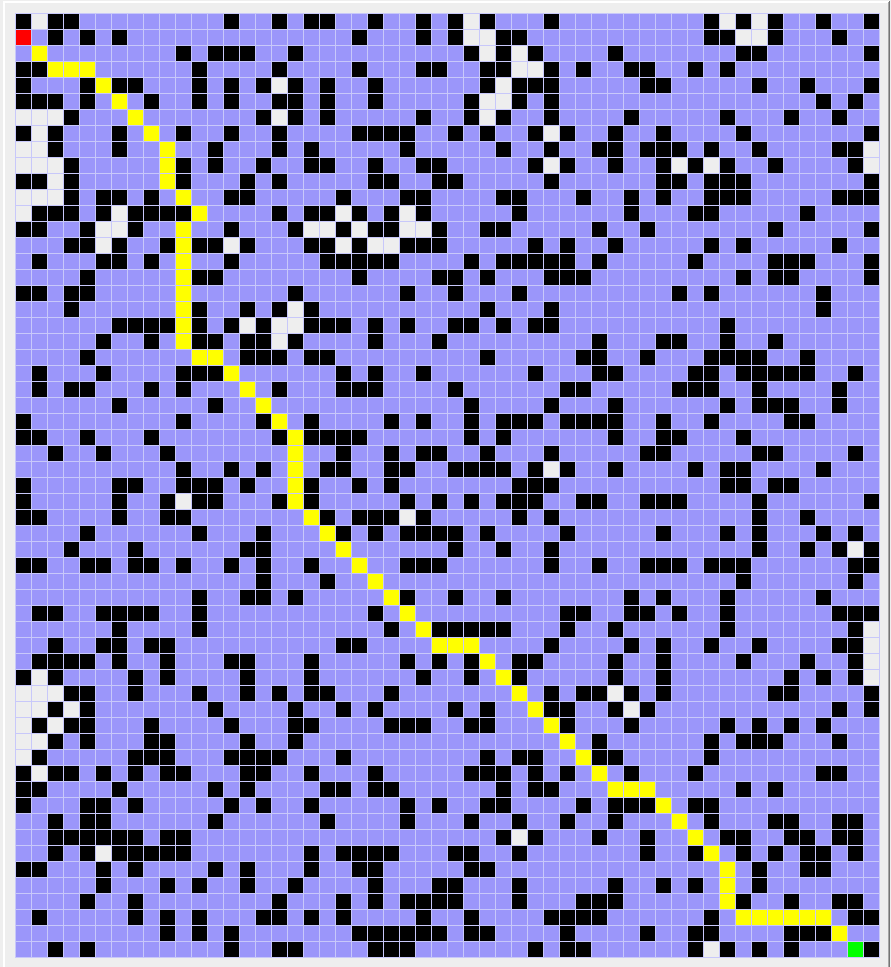
\includegraphics[width=0.4\textwidth]{djikstra.png}
\caption{Wizualizacja algorytmu Dijkstry \cite{searchpathsimplementations}}
\end{figure}

\begin{figure}
\label{fig:astar}
\centering
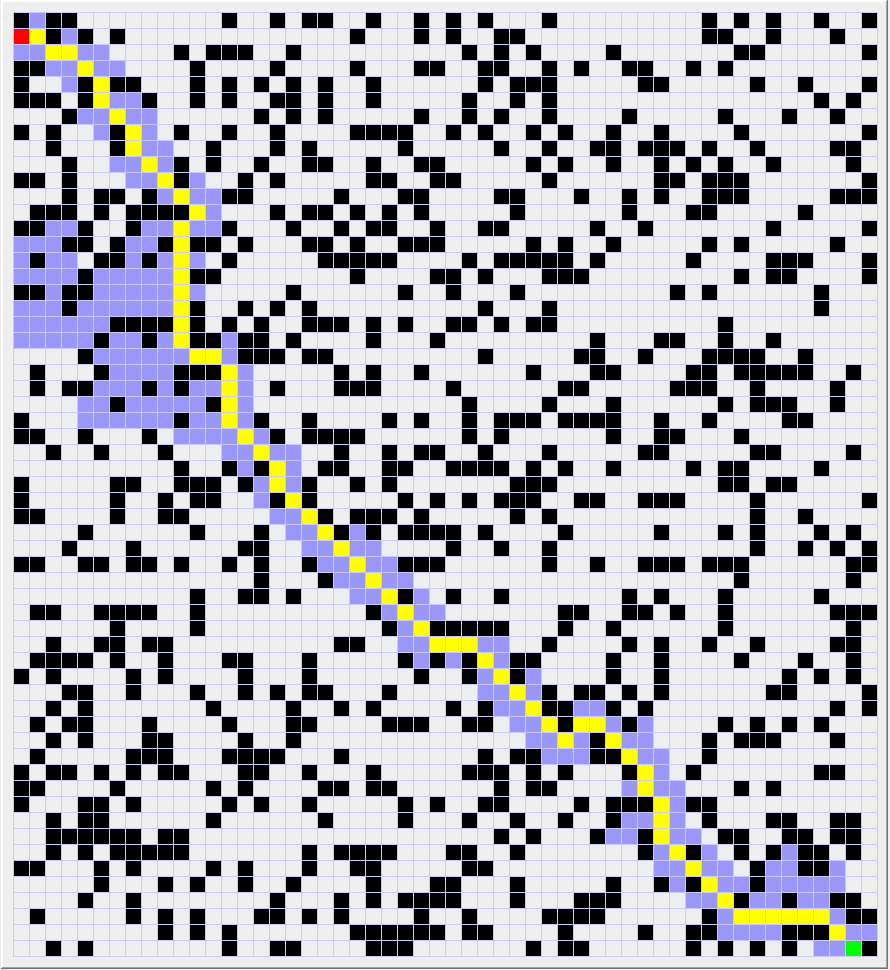
\includegraphics[width=0.4\textwidth]{astar.png}
\caption{Wizualizacja algorytmu A*, \cite{searchpathsimplementations}}
\end{figure}